
\documentclass[fleqn,addpoints]{exam}

\usepackage{graphicx}
\usepackage{float}
\usepackage{amsmath}
\usepackage{cancel}
\usepackage{polynom}
\usepackage{caption}

\printanswers

\ifprintanswers 
\usepackage{2in1, lscape} 
\fi

\title{Math 115 \\ Homework 18}
\date{April 16, 2011}

\begin{document}

\maketitle

% \begin{figure}[H]
%   \centering
%   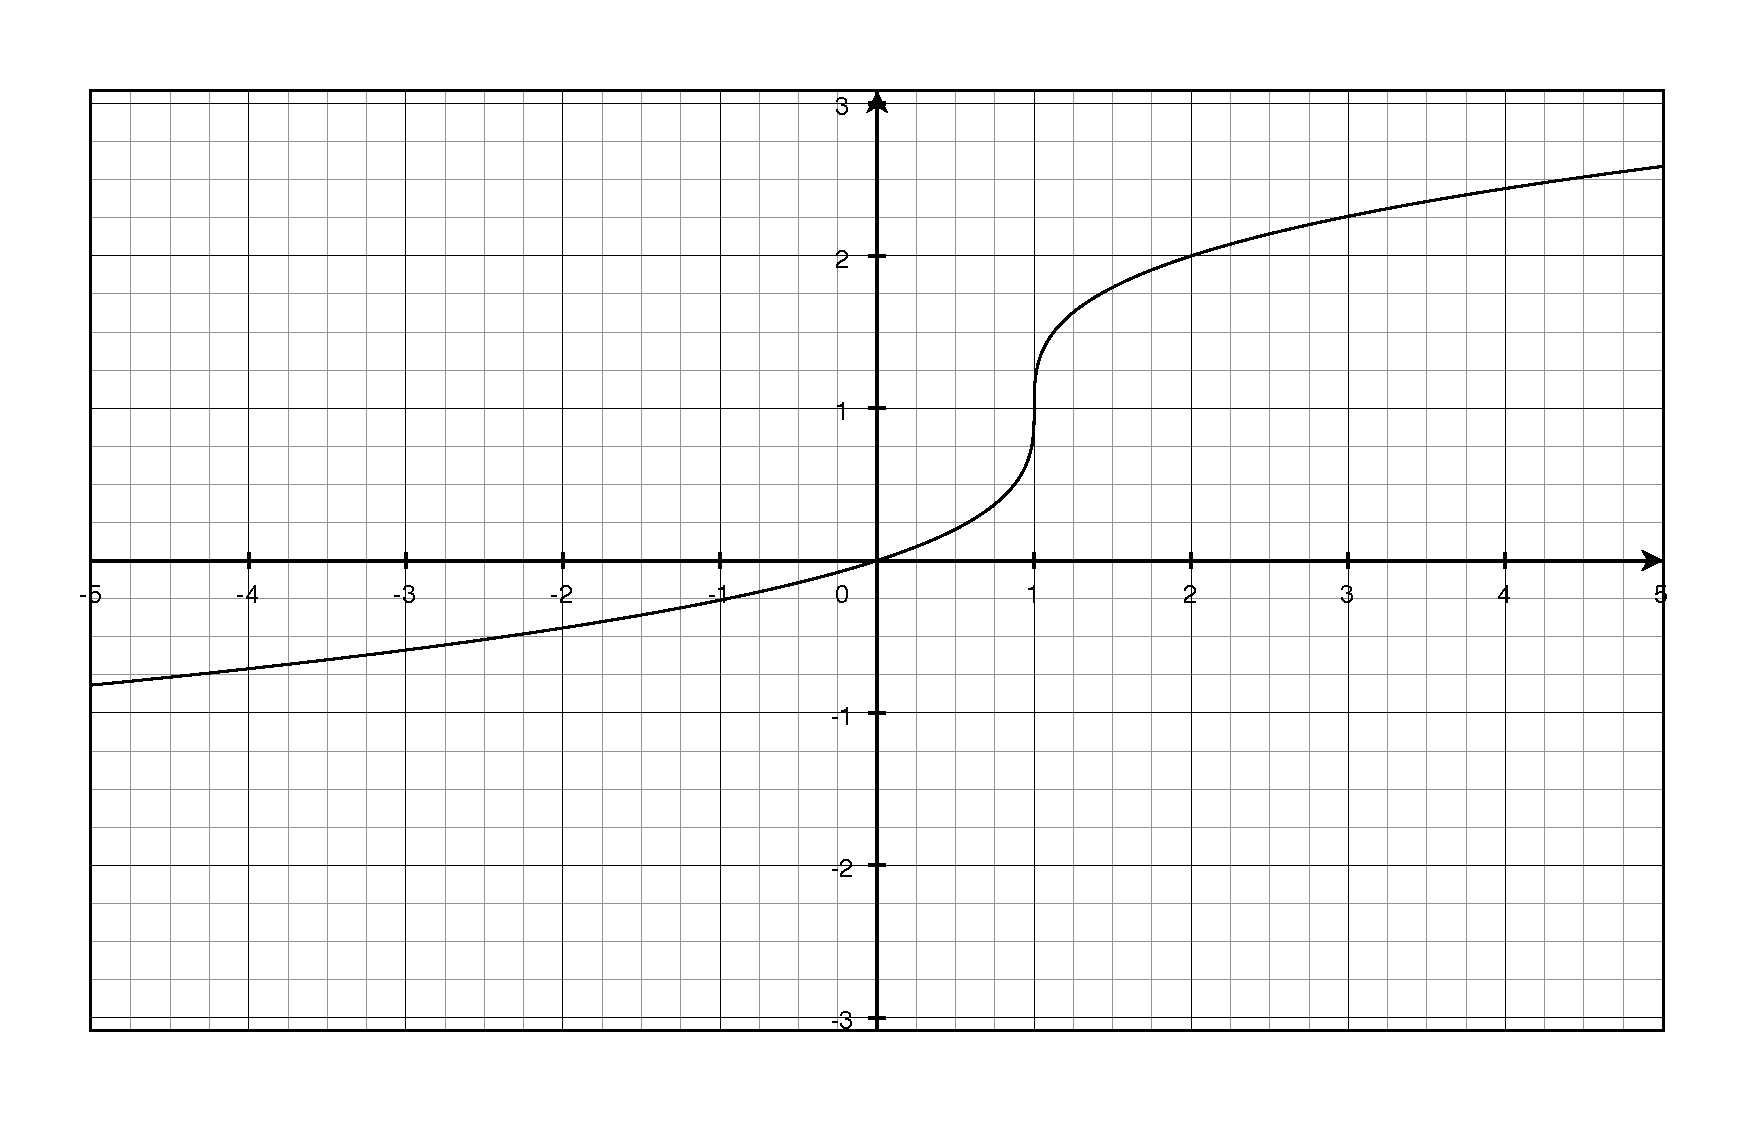
\includegraphics[scale=.3]{question7.eps}
%   \caption*{Question 7}
% \end{figure}

\section{Administrative}

The Chapter 3 exam will be next Tuesday, April 19.  

\section{Homework}

\begin{itemize}
  \item Read Section 3.5
  \item pp 335-340: 1-6, 7, 11, 14, 17, 25-26, 31, 35, 38, 42, 43, 47, 54, 68-70
\end{itemize}

As usual, you can just leave the answer as $\dfrac{\ln 2}{3}$ (or whatever it is) if you don't have a calculator.

\section{Review}

You should do some of the review problems on pp 342-345 to prepare for the test.

\ifprintanswers

\section{Homework}

For these problems, it's useful to have a general equation for the time to multiply by a factor of x in terms of the rate.  Here's what it is:
\begin{align*}
  xP &= P e^{rt} \\
  x &= e^{rt} \\
  \ln x &= rt \\
  t &= \frac{\ln x}{r} \\
\end{align*}

So if you want $x$ times as much money and you have interest rate $r$, you need to wait for $\frac{\ln x}{r}$ years.

\begin{description}

\item[1] c
\item[2] e
\item[3] b
\item[4] a
\item[5] d
\item[6] f

\item[7]

After 10 years:
\[
  A = 1000 e^{.12 \cdot 10} \approx 3320.12 \\
\]

Time to double:
\[
  t = \frac{\ln 2}{.12} \approx 5.78
\]

\item[11]
Annual rate:
\begin{align*}
  1505 &= 500 e^{10r} \\
  \frac{1505}{500} &= e^{10r} \\
  10r &= \ln 1505 - \ln 500 \\
  r &= \frac{\ln 1505 - \ln 500}{10} \\
  r &\approx .11
\end{align*}

Time to double:
\[
  t = \frac{\ln 2}{.11} \approx 6.29
\]

\item[14]
Initial investment:
\begin{align*}
  20000 &= P e^{.08 \cdot 10} \\
  P &= \frac{20000}{e^{0.8}} \\
  P &\approx 8986.58
\end{align*}

Time to double:
\[
  t = \frac{\ln 2}{.08} \approx 8.67
\]

\item[17]
For everything other than continuous:
\begin{align*}
  2P &= P(1 + \frac{r}{n})^{nt} \\
  2 &= (1 + \frac{r}{n})^{nt} \\
  \ln 2 &= \ln (1 + \frac{r}{n})^{nt} \\
  \ln 2 &= nt \ln (1 + \frac{r}{n}) \\
  t &= \frac{\ln 2}{n \ln (1 + \frac{r}{n})} \\
\end{align*}

For continuous:
\begin{align*}
  2P &= P e^{rt} \\
  2 &=  e^{rt} \\
  \ln 2 &= rt \\
  t &= \frac{\ln 2}{r} \\
\end{align*}

Plugging in the actual numbers
\begin{description}
\item[a]
6.642

\item[b]
6.330

\item[c]
6.302

\item[d]
6.301

\end{description}

% \item[19]
% \begin{tabular}{|c||c|c|c|c|c|c|}
%   \hline
%   r & 2\%   & 4\%  & 6\%  & 8\%  & 10\& & 12\% \\
%   \hline
%   t & 54.9 & 27.5 & 18.3 & 13.7 & 11.0 & 9.2  \\
%   \hline  
% \end{tabular}



\item[25]
\[
  r = \frac{\ln 2}{1620} \approx 0.00043
\]

After 1000 years:
\[
  A = 10 e^{-.00043 * 1000} \approx 6.5
\]

\item[26]
From question 25, the rate is .00043

Initial quantity
\begin{align*}
  1.5 &= A e^{-.00043 * 1000} \\ 
  1.5 &= A e^{-0.43} \\
  A &= 1.5 \cdot e^{0.43} \\
  A &\approx 2.3 \\
\end{align*}

\item[31]
We know that the equations is going to look like $y=ae^{bx}$ and we need to find $a$ and $b$.  With two points, we can
make two equations:

If we plug in the first point, we can find $a$:
\begin{align*}
  1 &= ae^{0x} \\
  a &= 1 \\ 
\end{align*}

Then we can use the second point to find $b$:
\begin{align*}
  10 &= 1 \cdot e^{3b} \\ 
  3b &= \ln 10 \\ 
  b &= \frac{\ln 10}{3} \\ 
  b &\approx 0.768 \\
\end{align*}

So the final equations is: $y = e^{.768x}$.  Since $e^{\ln 10/3} = 10^{1/3}$, another equation that would work is:
$y = 10^{x/3}$.

\item[35]
\begin{align*}
  150000 &= 105300 e^{0.015t} \\
  1500 &= 1053 e^{0.015t} \\
  \frac{1500}{1053} &=  e^{0.015t} \\
  0.015t &= \ln \frac{1500}{1053} \\
  t &= \frac{1}{0.015} \cdot \ln \frac{1500}{1053} \\
  t &\approx 23.6
\end{align*}

So the population of 150,000 will be reached about July, 2023.

\item[38]
This is a case where a negative time makes sense, because it can represent a time in the past.  So 1960 is represented by $t = -40$.
\begin{align*}
  100250 &= 140500 e^{-40k} \\
  \frac{100250}{140500} &= e^{-40k} \\
  \ln \frac{10025}{14050} &= -40k \\
  k &\approx .00843 \\
\end{align*}

In 2020, the population will be: $140500 e^{0.00843 \cdot 20} \approx 166330$.

\item[42]
\[
  r = \frac{\ln 2}{1620} \approx 0.000428
\]

\begin{align*}
  A &= A_0 e^{-0.000428 \cdot 100} \\
  \frac{A}{A_0} &\approx 0.96 \\
\end{align*}

96\% remains after 100 years.

\item[43]
\[
  r = \frac{\ln 2}{5730} \approx 0.000121
\]

\begin{align*}
  .15 A_0 &= A_0 e^{-0.000121 t} \\
  .15  &= e^{-0.000121 t} \\
  \ln .15  &= -0.000121 t \\
  t &= - \frac{\ln .15}{0.000121} \\
  t &\approx 15679 \\
\end{align*}

\item[47]

\begin{description}
\item[a]
\begin{align*}
  300000 &= \frac{500000}{1 + 0.6 e^{12k}} \\
  3 &= \frac{5}{1 + 0.6 e^{12k}} \\
  3 + 1.8 e^{12k} &= 5 \\
  1.8 e^{12k} &= 2 \\
  e^{12k} &= 1.11 \\
  k &\approx 0.053 \\
\end{align*}

\item[b]
280,771

\end{description}

\item[54]

\begin{description}
\item[a] 
\[
  10 \log \frac{10^{-10}}{10^{-12}} =   10 \log 10^2 = 20 
\]

\item[b] 
\[
  10 \log \frac{10^{-5}}{10^{-12}} =   10 \log 10^7 = 70
\]

\item[c] 
\[
  10 \log \frac{10^{-2.5}}{10^{-12}} =   10 \log 10^{9.5} = 95
\]

\item[d] 
\[
  10 \log \frac{10^{0}}{10^{-12}} =   10 \log 10^{12} = 120
\]

\end{description}

\item[68]
false

\item[69]
false

\item[70]
false (it's actually shifted up)

\end{description}

\else

\vspace{3 in}

{\em It is better to vote for what you want and not get it than to vote for what you don't want and get it.}

\vspace{.1 cm}
\hspace{1 cm} --Eugene Debs
\fi
\end{document}

